\documentclass[a4paper,11pt, twocolumn]{article}
\usepackage[margin=0.8in]{geometry}
\usepackage{xcolor}
\usepackage{graphicx} %package to manage images
\graphicspath{ {./images/} }

\title{AS-00 Basic Electrical Principles}
\author{Revision sheet}
\date{}

\usepackage{fancyhdr}
\pagestyle{fancy}
\fancyhead{} % clear all header fields
\renewcommand{\headrulewidth}{0pt} % no line in header area
\fancyfoot{} % clear all footer fields
\renewcommand{\footrulewidth}{0.4pt}
\fancyfoot[C]{\thepage} % page number in "outer" position of footer line
\fancyfoot[R]{\footnotesize Thomas Boxall \\ Images from WJEC E-Book} % other info in "inner" position of footer line
\fancyfoot[L]{\footnotesize AS-00 Basic Electrical Principles \\ Revision sheet}


\begin{document}

\maketitle
\thispagestyle{fancy}

\section{Fundamental Units}
There are a number of fundamental units which are used commonly across the entirety of electronics.
\subsection{Charge}
Charge ($Q$) is measured in the Coulomb (C). 
\subsection{Current}
Current ($I$)  is the amount of charge flowing past a point in a circuit per second. it is measured in Amperes, Amps for short, (A).
\subsection{Potential Difference}
Potential difference, also known as Voltage ($V$), is measured in Volts (V). The potential difference between two points is defined as the energy dissipated when one columb of charge moves between two points. Voltage is always measured 'across' or 'between' two points. 
\subsection{Resistance}
Resistance ($R$) of a component depends on the resistivity of the material and its dimensions. It is measured in Ohms ($\Omega$). Resistance is caused by electron collisions. A thicker wire will result in a lower resistance whereas a longer or hotter wire will result in an increased resistance.
\subsection{Power}
Power ($P$) is energy transfer per second. it is measured in Watts (W). Components which remove energy from a circuit (usually resistors), are said to 'dissipate' power.

\section{Fundamental Equations}
\subsection{Current, Charge and Time}
$\displaystyle Current = \frac{Charge}{Time}$\\
$\displaystyle I=\frac{Q}{t}$\\
\subsection{Work, Charge and Voltage}
$\displaystyle Work = Charge \times Voltage$\\
$W=QV$
\subsection{Voltage, Current and Resistance}
$Voltage = Current \times Resistance$\\
$V=IR$
\subsection{Power, Energy and Time}
$\displaystyle Power = \frac{Energy}{Time}$\\
$\displaystyle P=\frac{E}{T}$
\subsection{Power, Current and Voltage}
$Power = Current \times Voltage$\\
$P=IV$
\subsection{Power, Current and Resistance}
$Power = Current ^{2} \times Resistance$\\
$P=I^2R$

\section{Circuit components}
\subsection{Resistors}
Resistors are very small and come in different series. Each series has a different tolerance and different decades. For this course, use the E24 series which is listed on the front cover of the formula book. To choose resistors, generally pick the E24 resistor which has a higher resistance value than the ideal value. 
\subsection{Voltmeter}
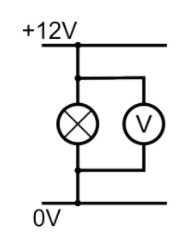
\includegraphics[width=0.3\textwidth]{voltmeter.jpg}\\
A voltmeter is connected in parallel with the component which you are measuring the voltage of.
\subsection{Ammeter}
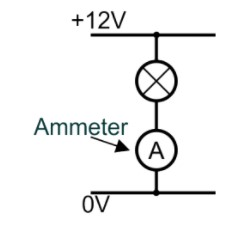
\includegraphics[width=0.3\textwidth]{ammeter.jpg}\\
An ammeter is connected in series with the component which you are measuring the current of.

\section{Circuit Styles}
\subsection{Series}
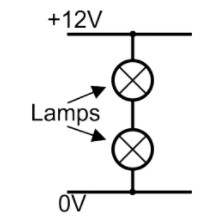
\includegraphics[width=0.3\textwidth]{series.jpg}\\
The current through the components is the same. The voltage is different across the components.
\subsection{Parallel}
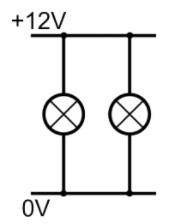
\includegraphics[width=0.3\textwidth]{parallel.jpg}\\
The current is split between the components. The voltage is the same across the components.

\section{Multiple resistor circuits}
\subsection{Resistors in Series}
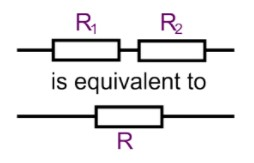
\includegraphics[width=0.3\textwidth]{resistorSeries.jpg}\\
$R_{total} = R_1 + R_2...$ This will work for any number of resistors.
\subsection{Resistors in Parallel}
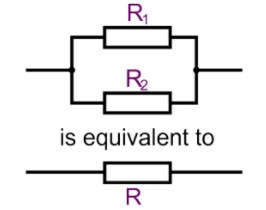
\includegraphics[width=0.3\textwidth]{resistorParallel.jpg}\\
$\displaystyle \frac{1}{R_{total}} = \frac{1}{R_1} + \frac{1}{R_2}...$ This works for any number of resistors, however if you just have two in a circuit, you can use the following formula:\\
$\displaystyle R_{total} = \frac{R_1 \times R_2}{R_1 + R_2}$

\section{Laws}
There are a number of key laws to understand with Electronics.
\subsection{Ohms Law}
The current through an ohmic conductor is directly proportional to the voltage at a constant temperature.\\
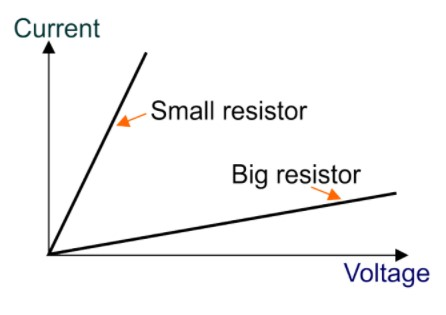
\includegraphics[width=0.3\textwidth]{ohmsLaw.jpg}\\
Non-Ohmic conductors have curvy lines on the graph.
\subsection{Kirchhoff's Current Law}
\textit{The sum of the currents flowing into a node is zero.}\\
Or alternatively - The sum of the currents flowing into the nodes equals the sum of those flowing out.
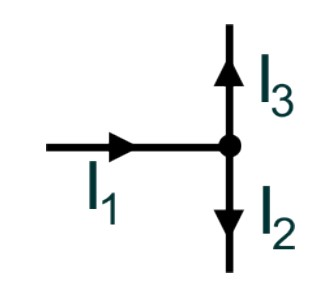
\includegraphics[width=0.3\textwidth]{kcl.jpg}\\
$I_1 = I_2+ I_3$
\subsection{Kirchhoff's Voltage Law}
\textit{The sum of voltage around a closed loop is zero.}\\
Or alternatively - The sum of voltages across components in series is equal to the total voltage across them.
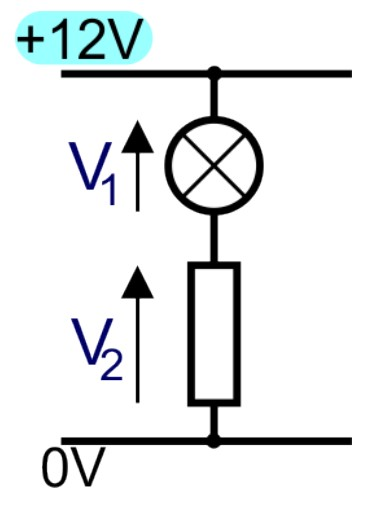
\includegraphics[width=0.3\textwidth]{kvl.jpg}\\
$V_1 + V_2 = 12\mathrm{V}$

\section{Potential Dividers}
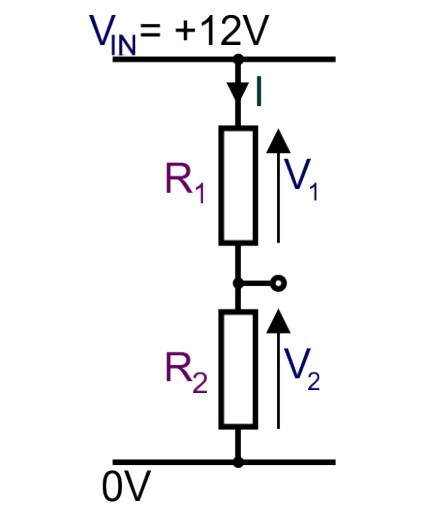
\includegraphics[width=0.3\textwidth]{potDev.jpg}\\
Two resistors connected in series and a power supply divides the voltage between them in the ratio of the resistors. As seen in the diagram above $V_{IN} = V_1+V_2$. To work out what $V_1$ and $V_2$ are, use the following equations respectively $\displaystyle V_1 = \frac{R_1}{R_1 + R_2}\times V_{IN}$\\
$\displaystyle V_2 = \frac{R_2}{R_1 + R_2}\times V_{IN}$
\subsection{Potentiometers}
A potentiometer is a three terminal resistor with a sliding or turning contact, that forms an adjustable voltage divider. There are two types - rotary and linear.

\section{Sensing Circuits}
Sensors are quite often needed as inputs to electronic systems. There are a few key types.
\subsection{Light Dependent Resistor}
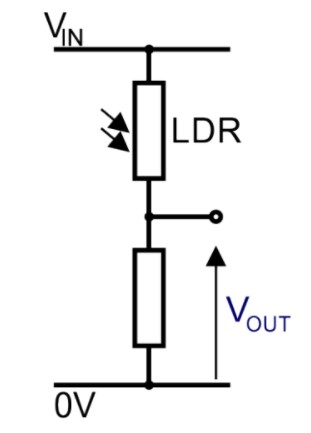
\includegraphics[width=0.3\textwidth]{ldr.jpg}\\
As the light levels increase, the resistance decreases. In the arrangement above, as the light which is shining on the LDR gets brighter, $V_{out}$ increases. If the resistor and LDR were the other way around: as the light shining on the LDR gets brighter, $V_{out}$ decreases. 
\subsection{Thermistor}
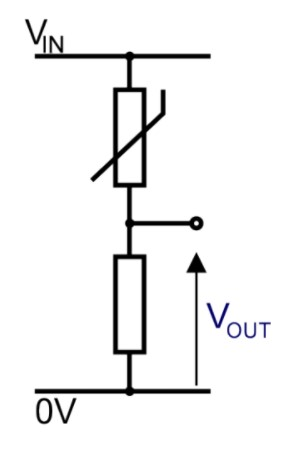
\includegraphics[width=0.3\textwidth]{thermistor.jpg}\\
There are two types of thermistors, Negative Temperature Coefficient (NTC) and Positive Temperature Coefficient (PTC). NTC is standard and will be most commonly used.\\
For the diagram above, as the temperature increases, $V_{out}$ increases. If the resistor and LDR were the other way around, as the temperature increased, $V_{out}$ would decrease.
\subsection{Adding a Sensitivity Control}
To add a Sensitivity control, replace the fixed resistor with a variable one. By increasing the value of the variable resistor, you are decreasing the sensitivity of the circuit.

\section{Thevenin's Theorem}
Any combination of power supplies and linear components (resistors) can be replaced by a single ideal voltage source and a single ideal resistor connected in series. Thevenin's theorem is used to simplify analysis of more complicated circuits as it reduces the number of linear components. They are always drawn the same\\
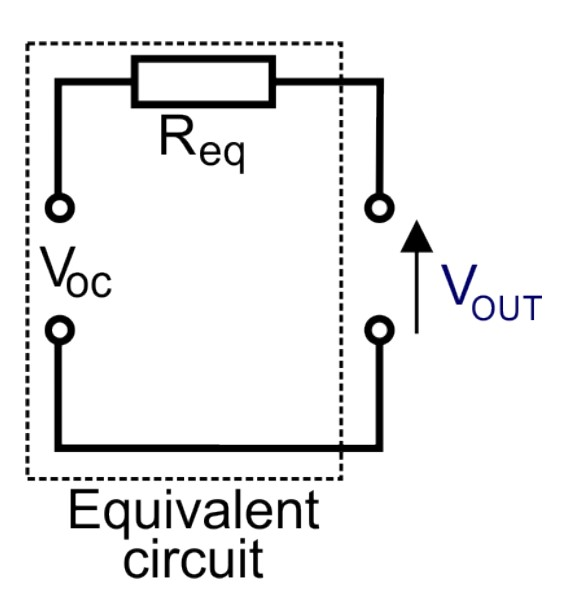
\includegraphics[width=0.3\textwidth]{thevenin.jpg}\\
There are a number of steps to go through to turn a circuit into a Thevenin equivalent circuit.
\begin{enumerate}
    \item Calculate $V_{OC}$ (Open circuit voltage which is the output voltage with no load connected).
    \item Calculate $I_{SC}$ (Short Circuit Current which is the current that flows then the output is short circuited).
    \item Calculate $R_{EQ}$ (Thevenin Resistance)\\ $\displaystyle R_{EQ} = \frac{V_{OC}}{I_{SC}}$
\end{enumerate}

\section{Loading}
Loading is an undesirable side effect. Connecting the load causes a voltage drop, we have loaded the power supply too much for it to be able to continue to output the expected output.\\
When connecting a low resistance load to a voltage source, the output voltage drops (loading). To avoid this, the source resistance needs to be much lower than the load. As a general rule $R_{LOAD} > 10 \times R_{SOURCE}$.

%Circuit Components
    %Voltmeters and ammeters
%Series and parallel
%Resistors and adding them together
%Laws
    %ohms
    %KCL
    %KVL
%Potential Dividers
    %potentiometers
%Sensing Circuits
%Thevenins theorem


\end{document}
